\section{Ergebnisse aus der Literaturrecherche}\label{chap:results_lit}

Das folgende Kapitel fasst die Ergebnisse der systematischen Literaturanalyse zusammen (vgl. Tabelle~\ref{tab:literatur}). Dabei werden die in Kapitel~\ref{chap:kriterienkatalog} definierten Kriterien auf die identifizierten Publikationen angewendet.

\vspace{1em}

Insgesamt umfasst die Analyse 151 Veröffentlichungen, die in Tabelle~\ref{tab:literatur} aufgeführt sind. Abbildung~\ref{fig:1-veroeffentlichungen-jahr} zeigt die jährliche Verteilung der Publikationen. Von den insgesamt 151 Arbeiten wurden 58 im Zeitraum von 2020 bis 2025 veröffentlicht, was einem Anteil von ca. 38~\% entspricht, während weitere 55~\% der Publikationen in den Jahren 2000 bis 2020 erschienen.

\begin{figure}[!htbp]
    \centering
    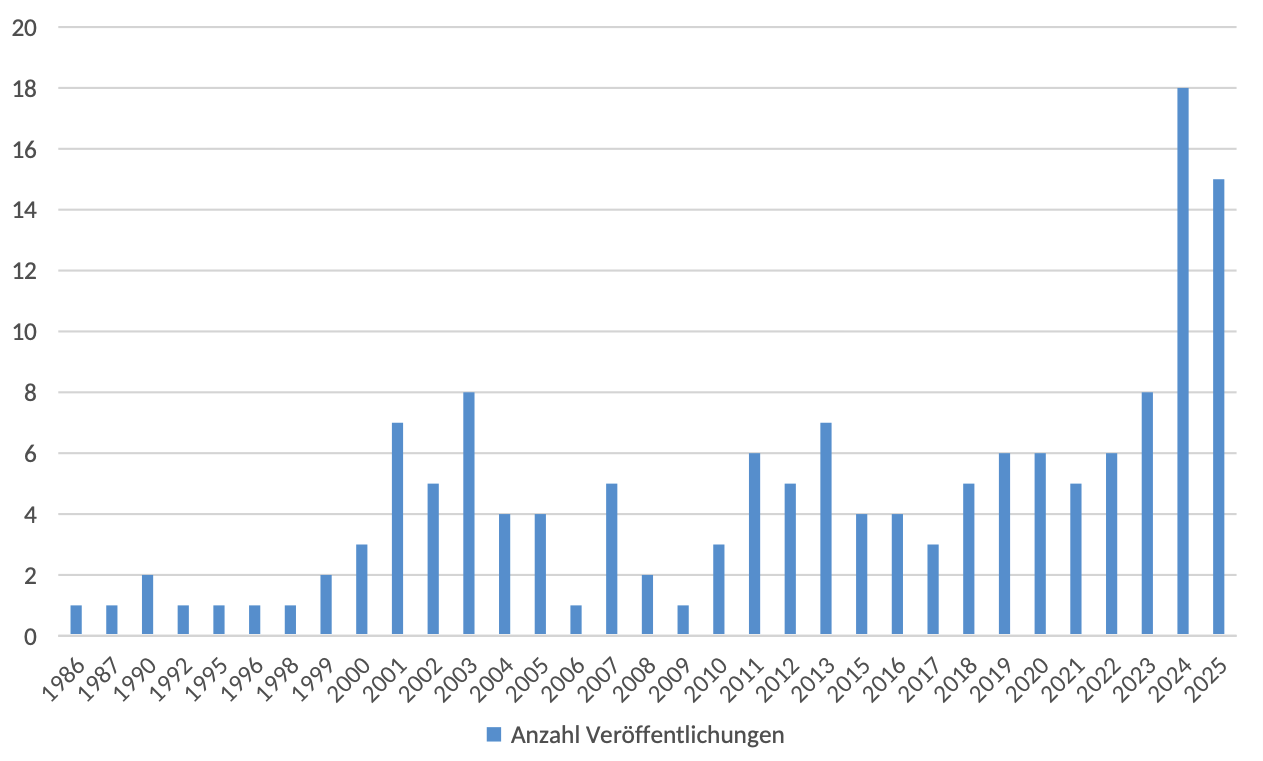
\includegraphics[width=0.90\textwidth]{graphics_lit/1-veroeffentlichungen-jahr.png}
    \caption{Übersicht der Veröffentlichungen pro Jahr}
    \label{fig:1-veroeffentlichungen-jahr}
\end{figure}

Aus Abbildung~\ref{fig:2-typ} ist ersichtlich, dass insgesamt 98~\% der Veröffentlichungen auf Journalartikel (ca. 36~\%) und Konferenzbeiträge (ca. 62~\%) entfallen. Während Journalartikel in Fachzeitschriften mit ausführlicherem Begutachtungsprozess erscheinen, werden Konferenzbeiträge überwiegend in Tagungsbänden veröffentlicht und dienen der schnellen Verbreitung aktueller Forschungsergebnisse \cite{abbadia_conference_2022}. Beide Publikationstypen sind daher für eine Trendanalyse sowie zur Ableitung von Best Practices geeignet.

\begin{figure}[!htbp]
    \centering
    % --- linke Seite: Grafik ---
    \begin{subfigure}[b]{0.48\textwidth}
        \centering
        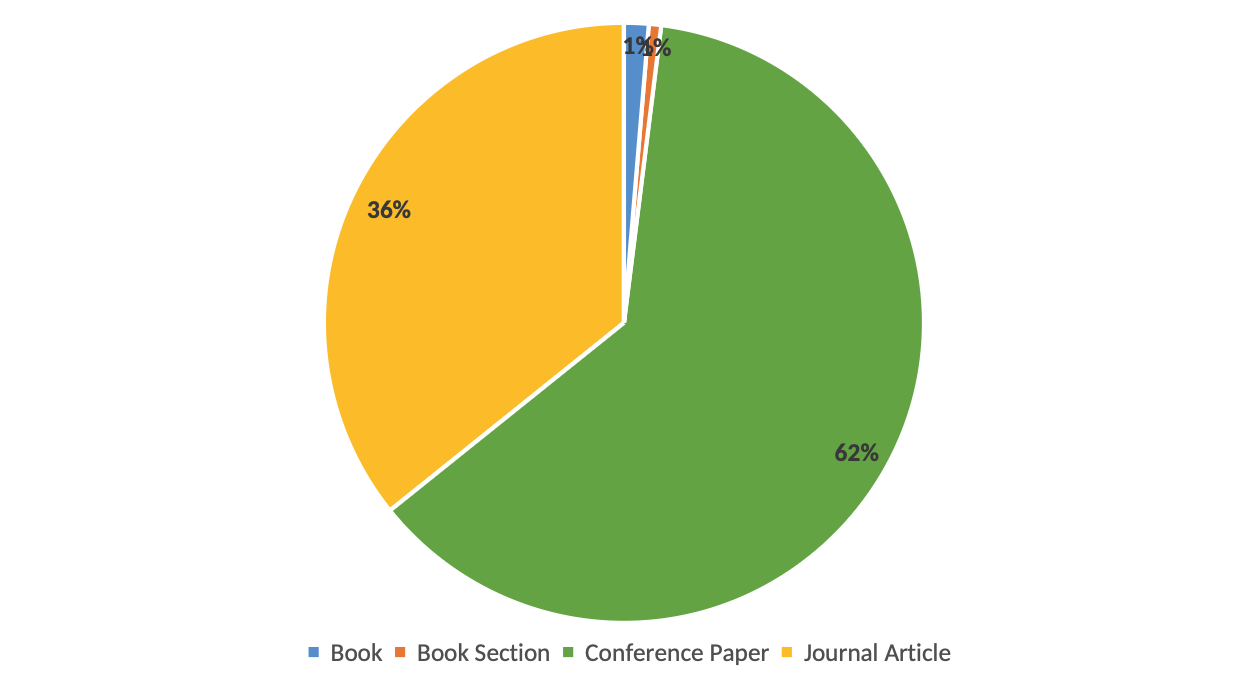
\includegraphics[width=1\textwidth]{graphics_lit/2-typ.png}
        \caption{Übersicht des Typs} 
        \label{fig:2-typ}
    \end{subfigure}
    \hfill
    % 
    % --- rechte Seite: Tabelle ---
    \begin{subfigure}[b]{0.48\textwidth}
        \centering
        \tiny
        \begin{tabularx}{\textwidth}{X c}
            \hline
            \multicolumn{2}{l}{\textbf{Journals}} \\
            \hline
            IEEE Transactions on Education & 10 \\
            Computer Applications in Engineering Education & 7 \\
            Journal on Educational Resources in Computing & 7 \\
            \hline
            \multicolumn{2}{l}{\textbf{Konferenzen}} \\
            \hline
            Workshop on Computer Architecture Education & 8 \\
            ACM Technical Symposium on Computer Science Education & 7 \\
            Annual International Symposium on Computer Architecture & 6 \\
            \hline
        \end{tabularx}
        \caption{Meistgenutzte Journals und Konferenzen}
        \label{tab:2-typ-detail}
    \end{subfigure}
    %
    \caption{Informationen zum Typ der Publikationen}
    \label{fig:2-typ-gesamt}
\end{figure}

Tabelle~\ref{tab:2-typ-detail} bietet eine Übersicht über die Zeitschriften und Konferenzen, in denen die meisten der untersuchten Publikationen veröffentlicht wurden. Die drei genannten Zeitschriften vereinen 44~\% aller Journalartikel, während die drei aufgeführten Konferenzen rund 22~\% der Konferenzbeiträge ausmachen.

Abbildung~\ref{fig:3-anzahl-themen} verdeutlicht, dass die häufigsten Themen der untersuchten Publikationen \enquote{Prozessoren und Architekturen} (44~\%), \enquote{Speicher und Performance} (11~\%) sowie \enquote{Hardware und Logistik} (10~\%) sind. Diese drei Themen umfassen zusammen rund 70~\% aller Publikationen. Dicht darauf folgen die Themen \enquote{Grundlagen und Theorien} sowie \enquote{Programmierung} mit jeweils 9~\% der Arbeiten.

\begin{figure}[!h]
    \centering
    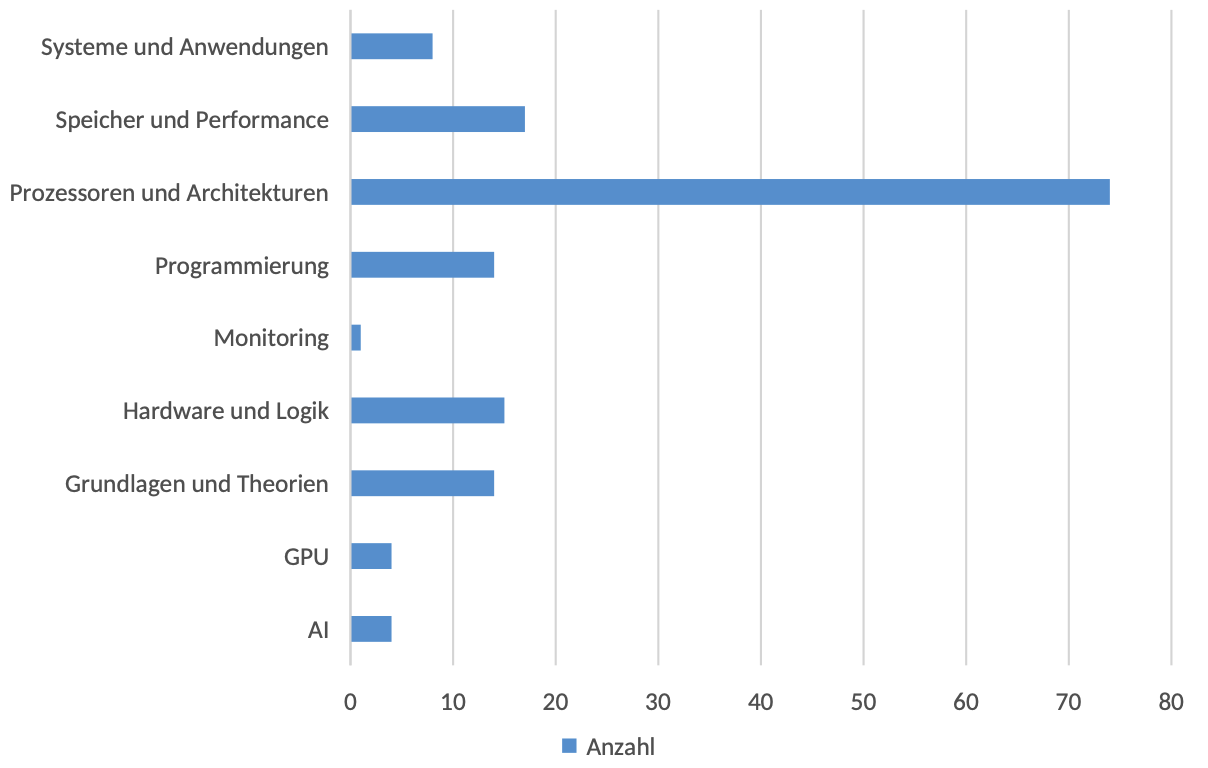
\includegraphics[width=0.90\textwidth]{graphics_lit/3-thema.png}
    \caption{Anzahl der Veröffentlichungen pro Thema}
    \label{fig:3-anzahl-themen}
\end{figure}

Eine detaillierte Untersuchung der drei am häufigsten vertretenen Themen ist in Abbildung~\ref{fig:4-top3-themen} dargestellt. Diese Grafik zeigt die Verteilung dieser Themen über verschiedene Zeitspannen. Die zugrunde liegenden Werte sind in der Tabelle~\ref{tab:themen-zeit} aufgeführt.

\begin{figure}[!htbp]
    \centering
    % --- linke Seite: Grafik ---
    \begin{subfigure}[b]{0.48\textwidth}
        \centering
        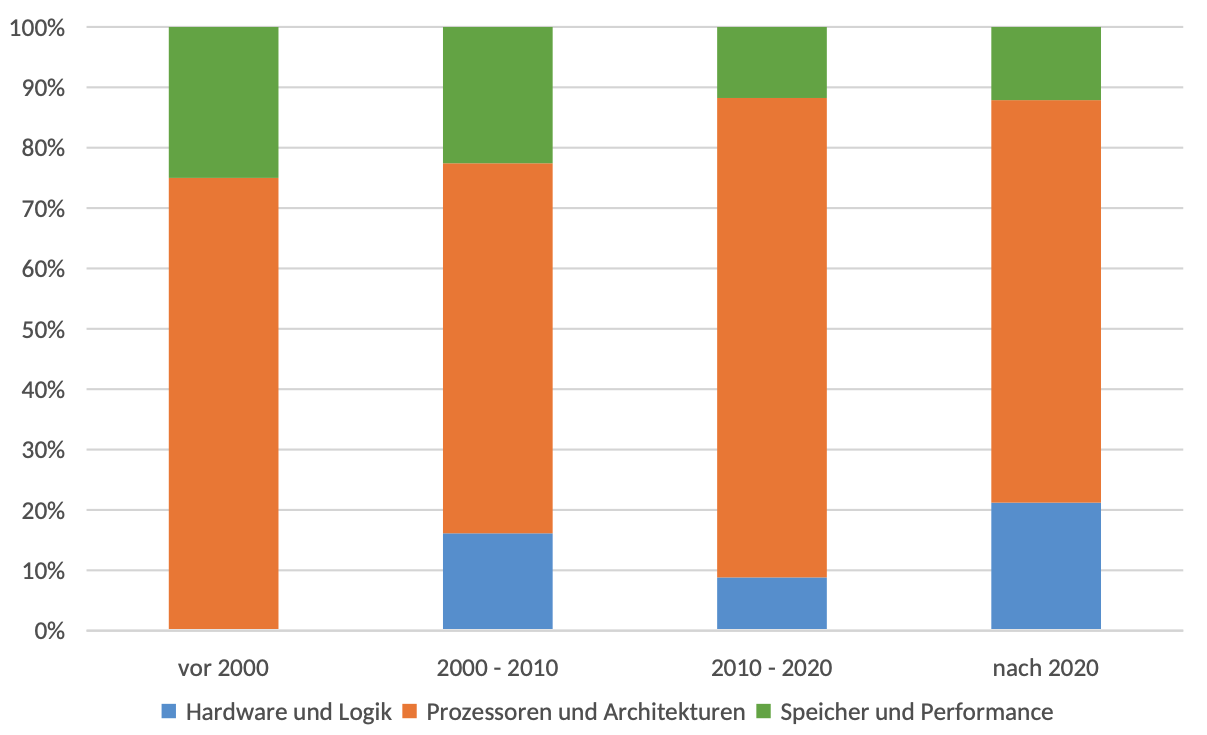
\includegraphics[width=0.90\textwidth]{graphics_lit/4-top3-themen-jahr.png}
        \caption{Jährliche Aufteilung Top 3 Themen (grafisch)}
        \label{fig:4-top3-themen}
    \end{subfigure}
    \hfill
    % 
    % --- rechte Seite: Tabelle ---
    \begin{subfigure}[b]{0.48\textwidth}
        \centering
        \tiny
        \begin{tabularx}{\textwidth}{lXXX}
            \hline
            \textbf{Zeitraum} & \textbf{Hardware und Logik} & \textbf{Prozessoren und Architekturen} & \textbf{Speicher und Performance} \\
            \hline
            vor 2000      & 0  & 6  & 2 \\
            2000--2010    & 5  & 19 & 7 \\
            2010--2020    & 3  & 27 & 4 \\
            nach 2020     & 7  & 22 & 4 \\
            \hline
        \end{tabularx}
        \caption{Jährliche Aufteilung Top 3 Themen (detailliert)}
        \label{tab:themen-zeit}
    \end{subfigure}
    %
    \caption{Jährliche Aufteilung Top 3 Themen}
    \label{fig:pub-typen}
\end{figure}

Für die Themen \enquote{Grundlagen und Theorien} sowie \enquote{Programmierung} zeigt Abb.~\ref{fig:5-top5-themen} die jährliche Verteilung. Die entsprechenden Werte sind in Tab.~\ref{tab:themen-zeit-2} aufgeführt. Auf eine detaillierte Analyse der verbleibenden Themen wir hier verzichtet. In dem Kapitel~\ref{chap:5-discussion} werde die Entwicklung aller Themen aufgegriffen und analysiert.

\begin{figure}[!htbp]
    \centering
    % --- linke Seite: Grafik ---
    \begin{subfigure}[b]{0.48\textwidth}
        \centering
        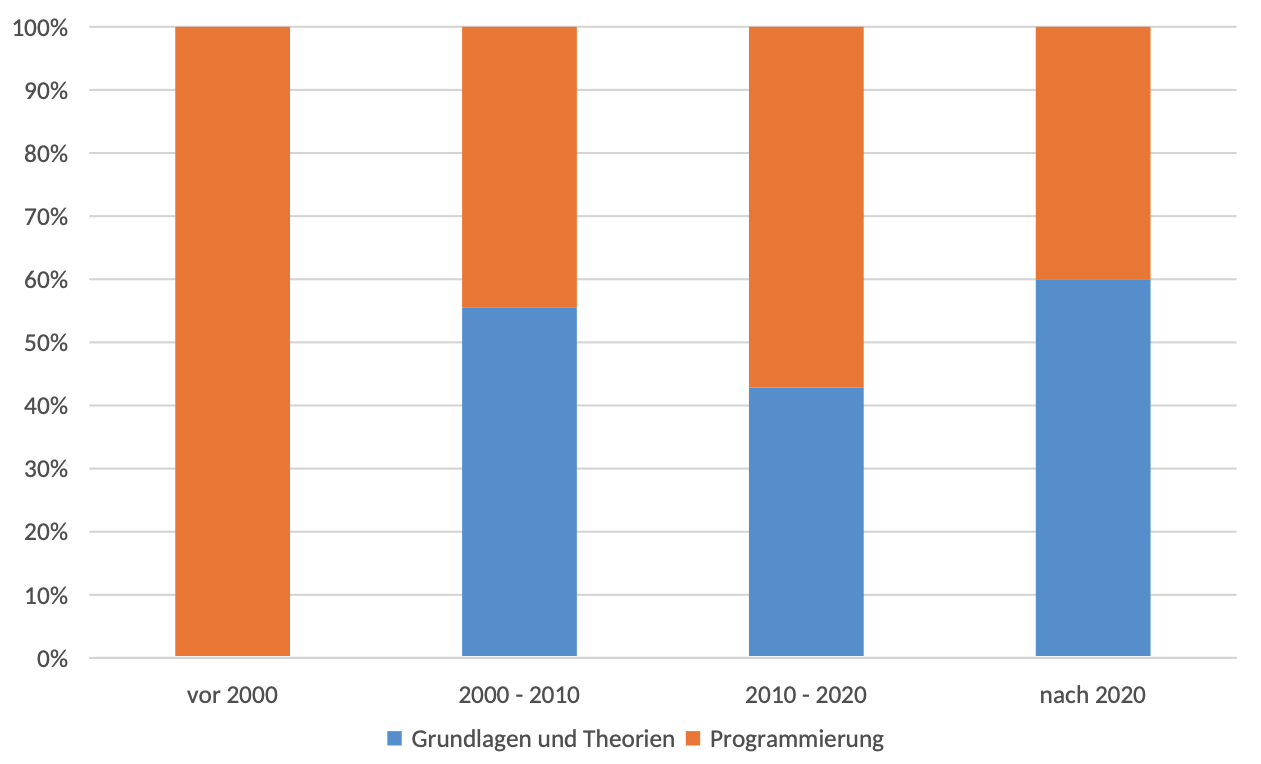
\includegraphics[width=0.90\textwidth]{graphics_lit/5-top5-themen-jahr.png}
        \caption{Jährliche Aufteilung weitere Themen (grafisch)}
        \label{fig:5-top5-themen}
    \end{subfigure}
    \hfill
    % 
    % --- rechte Seite: Tabelle ---
    \begin{subfigure}[b]{0.48\textwidth}
        \centering
        \tiny
        \begin{tabularx}{\textwidth}{lXX}
            \hline
            \textbf{Zeitraum} & \textbf{Grundlagen und Theorien} & \textbf{Programmierung} \\
            \hline
            vor 2000      & 0 & 2 \\
            2000--2010    & 5 & 4 \\
            2010--2020    & 3 & 4 \\
            nach 2020     & 6 & 4 \\
            \hline
        \end{tabularx}
        \caption{Jährliche Aufteilung weitere Themen (detailliert)}
        \label{tab:themen-zeit-2}
    \end{subfigure}
    %
    \caption{Jährliche Aufteilung weitere Themen}
    \label{fig:pub-typen}
\end{figure}

Hinsichtlich der Frage, ob die untersuchten Simulatoren spielerische Elemente (\textit{Gamification}) enthalten, bietet die Tabelle~\ref{tab:gamification} einen Überblick.

\begin{table}[!htbp]
    \centering
    \begin{tabular}{l r r}
        \hline
        \textbf{Gamification} & \textbf{Anzahl} & \textbf{\%} \\
        \hline
        Keine Elemente     & 145 & 96\% \\
        Elemente vorhanden & 6   & 4\%  \\
        \hline
        \textbf{Summe}     & 151 & 100\% \\
        \hline
    \end{tabular}
    \caption{Verteilung der Publikationen in Bezug auf enthaltene Gamification-Elemente}
    \label{tab:gamification}
\end{table}

Von den 151 Simulatoren der untersuchten wissenschaftlichen Publikationen wurden 15~\% als realitätsnah und 85~\% als didaktisch reduziert eingestuft. Die Verteilung bezogen auf die einzelnen Themenbereiche ist in Abbildung~\ref{fig:7-abstraktion-themen} dargestellt.

Die Abbildung~\ref{fig:8-abstraktion-jahr} verdeutlicht die zeitliche Entwicklung des Abstraktionslevels.

\begin{figure}[!htbp]
    \centering
    % --- linke Seite: Grafik ---
    \begin{subfigure}[b]{0.48\textwidth}
        \centering
        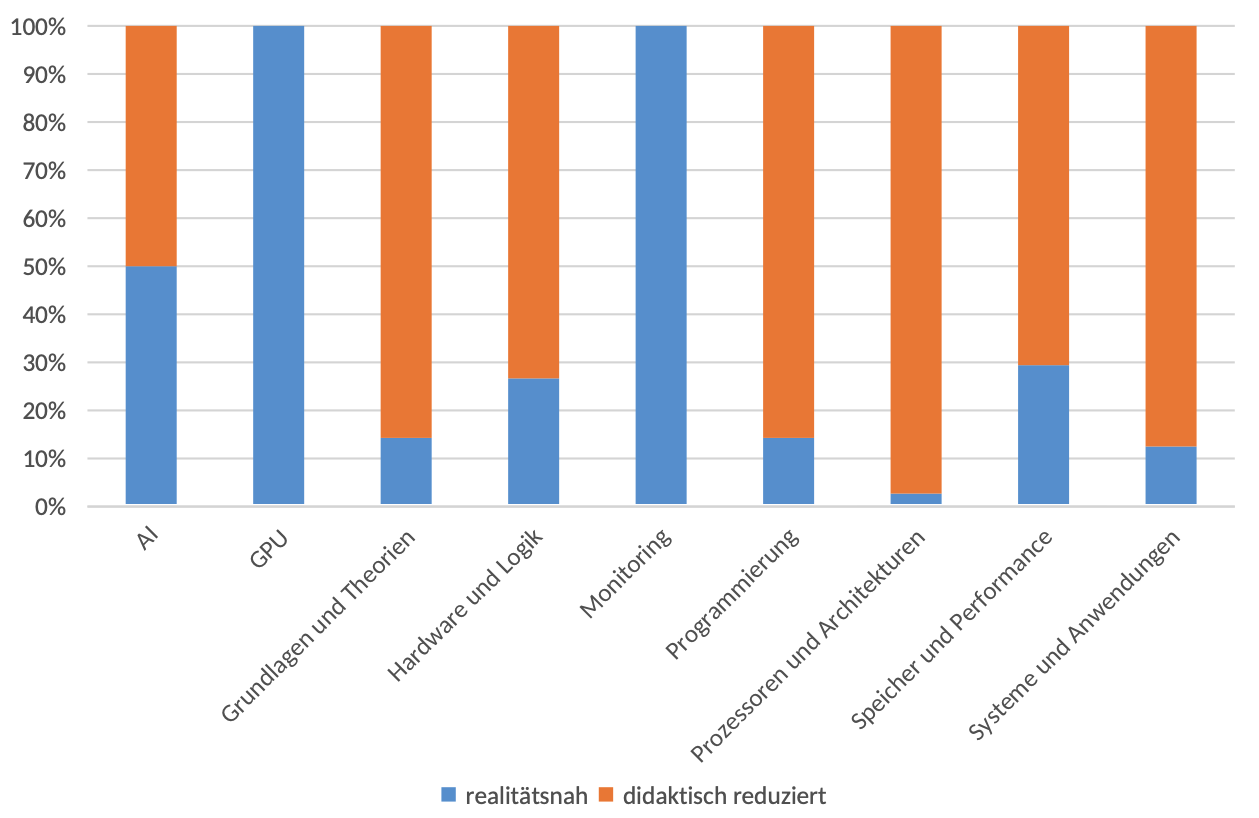
\includegraphics[width=0.90\textwidth]{graphics_lit/7-abtraktion-themen.png}
        \caption{Verteilung Abstraktionslevel auf Themen}
        \label{fig:7-abstraktion-themen}
    \end{subfigure}
    \hfill
    % 
    % --- rechte Seite: Grafik ---
    \begin{subfigure}[b]{0.48\textwidth}
        \centering
        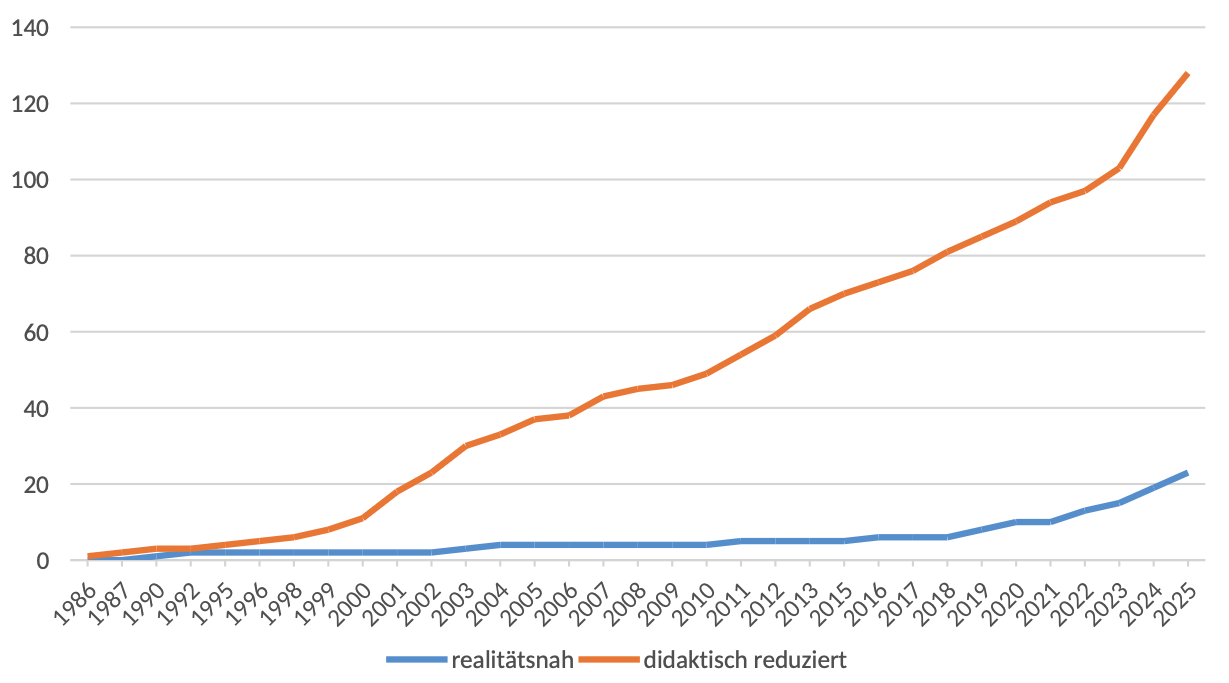
\includegraphics[width=0.90\textwidth]{graphics_lit/8-abstraktion-jahr.png}
        \caption{Zeitliche Entwicklung des Abstraktionslevels}
        \label{fig:8-abstraktion-jahr}
    \end{subfigure}
    %
    \caption{Analysen zum Abstraktionslevel}
    \label{fig:abstaktion-analysen}
\end{figure}

Anhand von Abbildung~\ref{fig:9-institution} ist zu erkennen, dass 89~\% der Publikationen die Hochschulbildung als Zielgruppe adressieren. 9~\% der untersuchten Simulatoren sind für Forschung und Beruf bestimmt, während sich die verbleibenden 2~\% auf schulische Bildung und Weiterbildungen aufteilen.

Untersucht man die Verteilung der Zielgruppen genauer, so zeigt Abbildung~\ref{fig:10-institution-themen} die Aufteilung der einzelnen Zielgruppen (\enquote{Schule}, \enquote{Hochschule}, \enquote{Forschung, Beruf}, \enquote{Weiterbildung}) auf die jeweiligen Themenbereiche. Dabei wird zum Beispiel deutlich, dass sich alle GPU-bezogenen Simulatoren der Forschungs- bzw. Berufsgruppe zuordnen lassen.

\begin{figure}[!htbp]
    \centering
    % --- linke Seite: Grafik ---
    \begin{subfigure}[b]{0.48\textwidth}
        \centering
        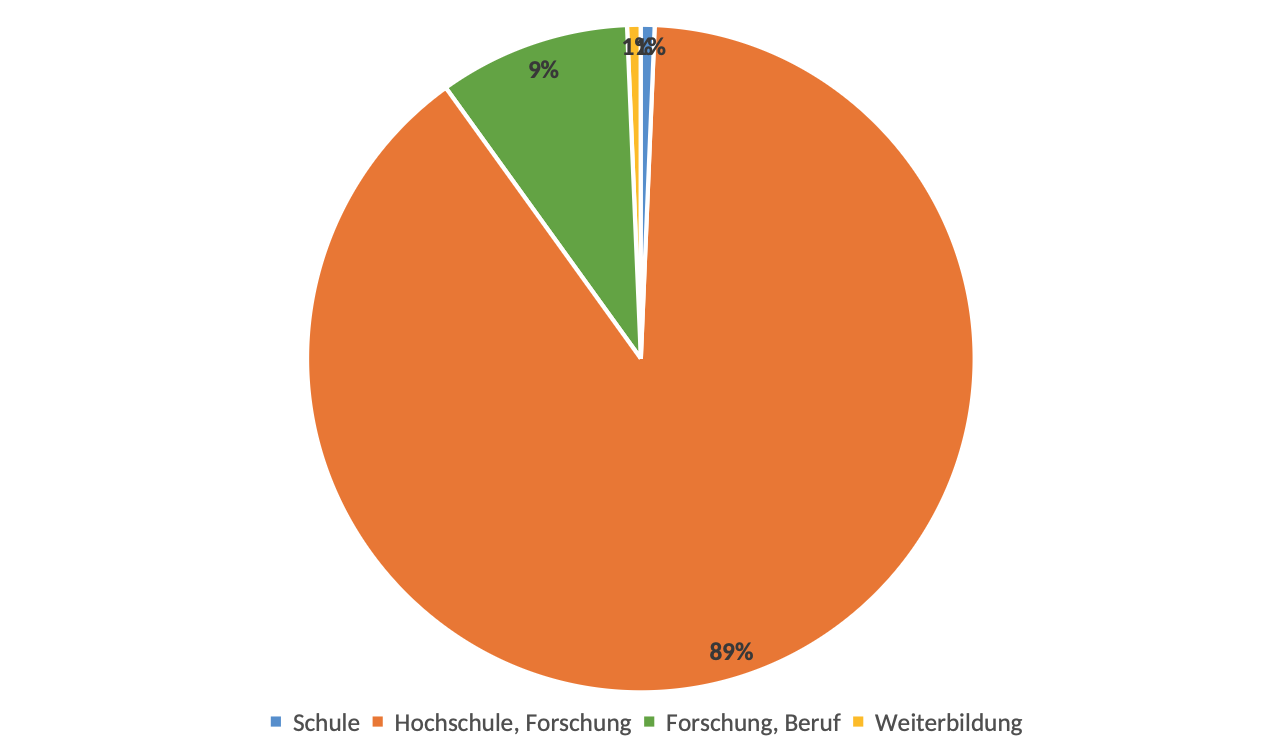
\includegraphics[width=0.90\textwidth]{graphics_lit/9-institution.png}
        \caption{Aufteilung Institutionen}
        \label{fig:9-institution}
    \end{subfigure}
    \hfill
    % 
    % --- rechte Seite: Grafik ---
    \begin{subfigure}[b]{0.48\textwidth}
        \centering
        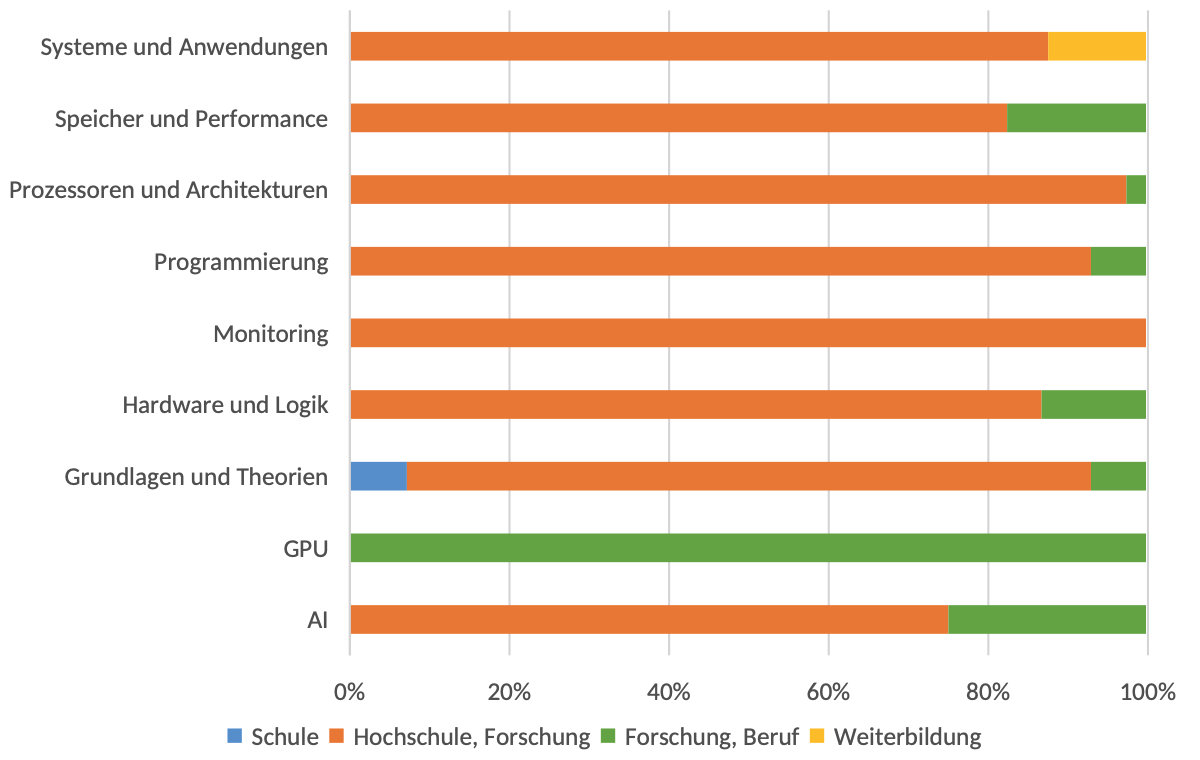
\includegraphics[width=0.90\textwidth]{graphics_lit/10-institution-themen.png}
        \caption{Aufteilung Institutionen nach Themen}
        \label{fig:10-institution-themen}
    \end{subfigure}
    %
    \caption{Analysen zu Institutionen}
    \label{fig:institution-analysen}
\end{figure}

Hinsichtlich des Zugriffs zeigt Abbildung~\ref{fig:11-zugriff} eine detaillierte Aufteilung. Die meisten Simulatoren (ca. 66~\%) sind offline nutzbar, während 11~\% entweder ausschließlich online oder sowohl online als auch offline verfügbar sind. In 19 Publikationen (ca. 13~\%) finden sich keine Angaben zur Art der Nutzung.

\begin{figure}[!htbp]
    \centering
    % --- linke Seite: Grafik ---
    \begin{subfigure}[b]{0.48\textwidth}
        \centering
        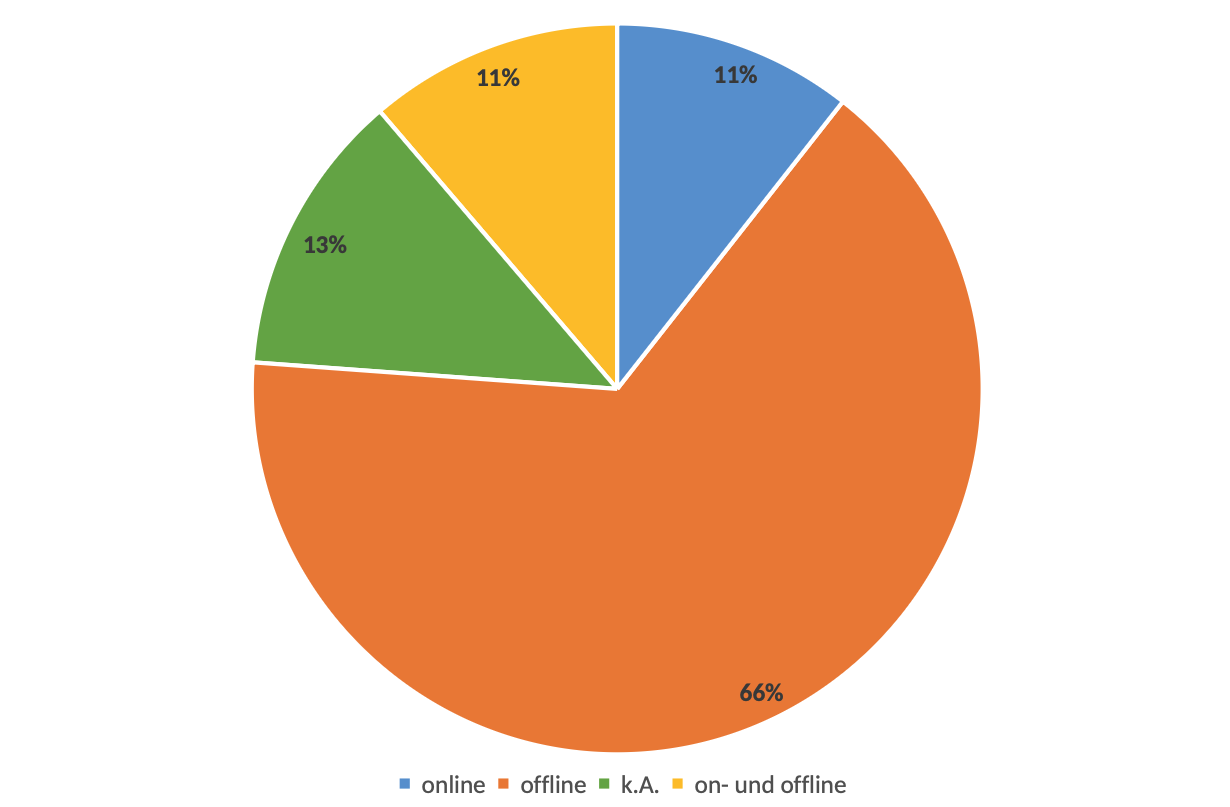
\includegraphics[width=0.90\textwidth]{graphics_lit/11-zugriff.png}
        \caption{Aufteilung Zugriff}
        \label{fig:11-zugriff}
    \end{subfigure}
    \hfill
    % 
    % --- rechte Seite: Grafik ---
    \begin{subfigure}[b]{0.48\textwidth}
        \centering
        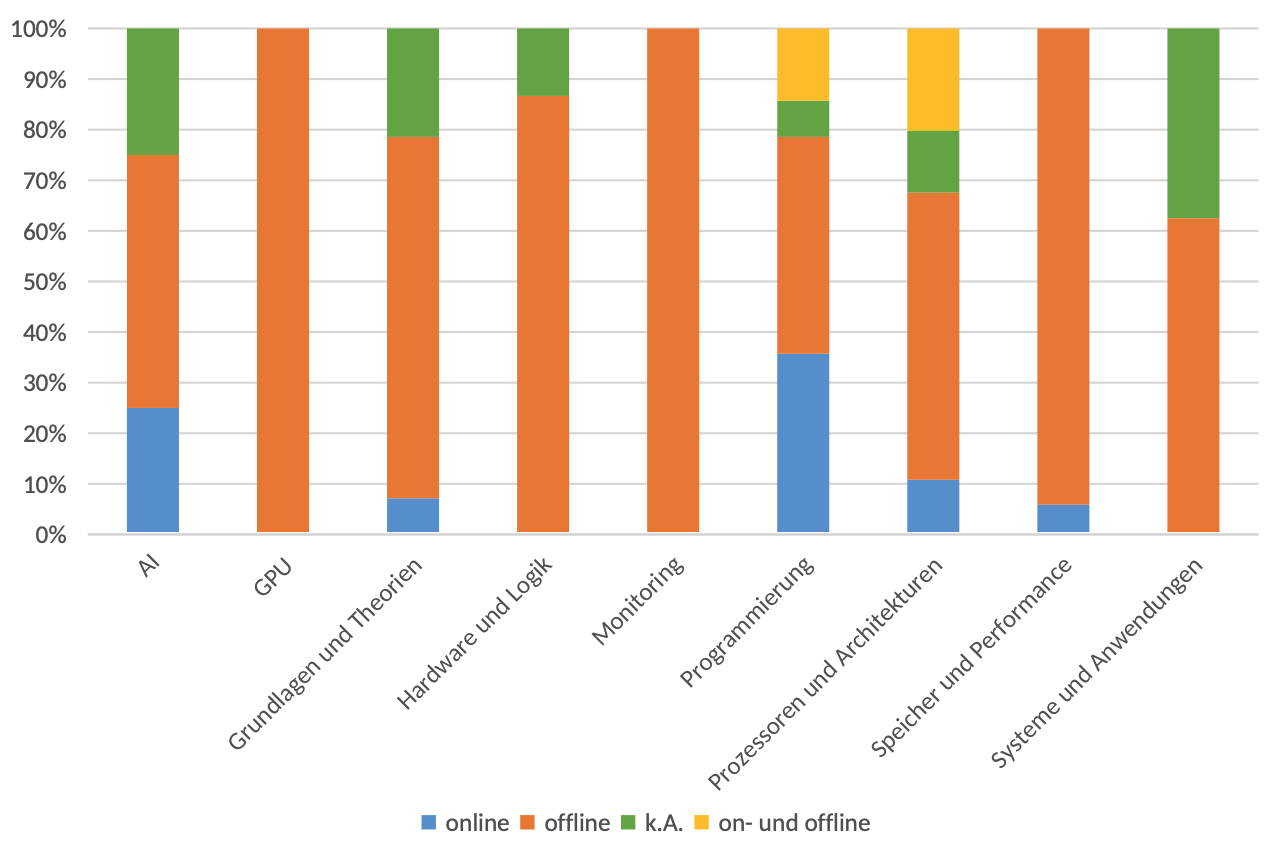
\includegraphics[width=0.90\textwidth]{graphics_lit/13-zugriff-thema.png}
        \caption{Zugriffsart pro Thema}
        \label{fig:13-zugriff-thema}
    \end{subfigure}
    %
    \caption{Analysen zu zum Zugriff}
    \label{fig:zugriff-analysen}
\end{figure}

Die zeitliche Verteilung der verschiedenen Zugriffsarten ist in Abbildung~\ref{fig:12-zugriff-jahr} dargestellt, die entsprechenden Werte sind in Tab.~\ref{tab:zugriff-zeit} aufgeführt.

\begin{figure}[!htbp]
    \centering
    % --- linke Seite: Grafik ---
    \begin{subfigure}[b]{0.48\textwidth}
        \centering
        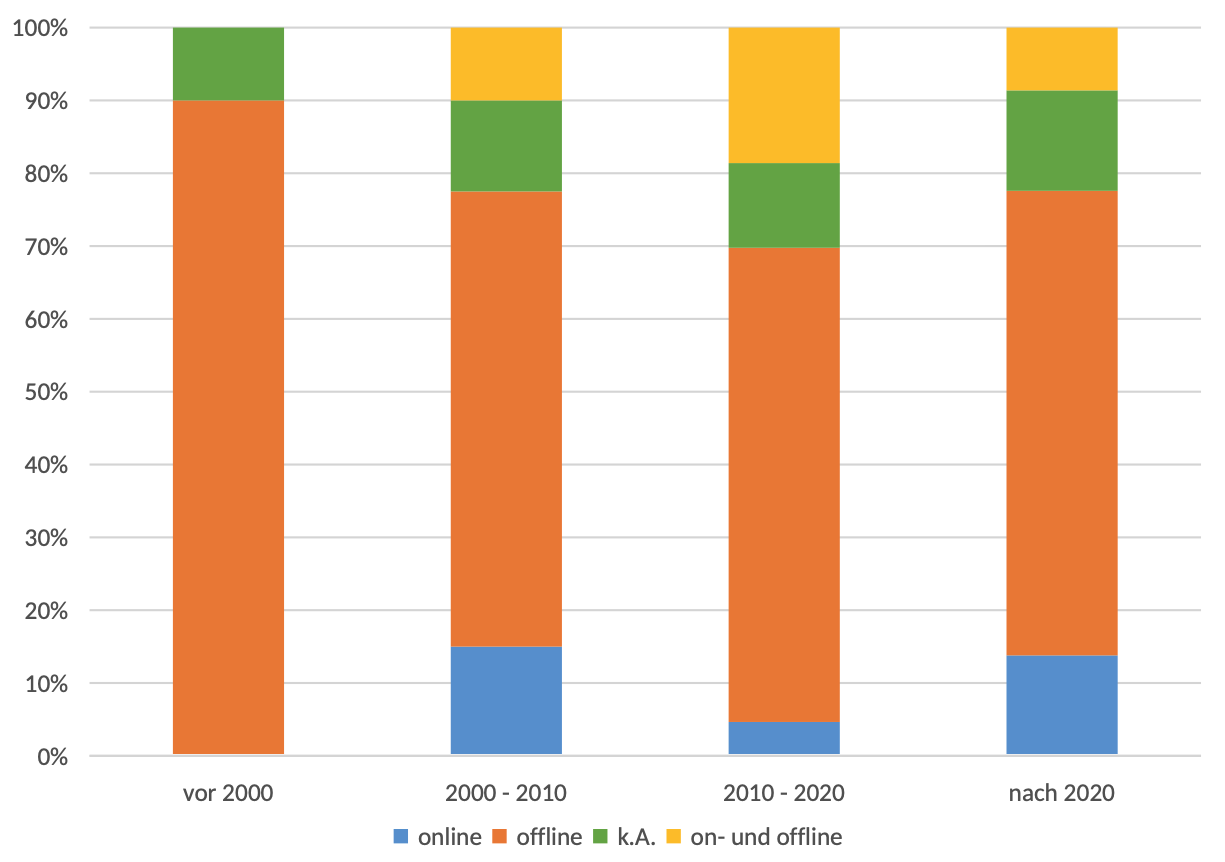
\includegraphics[width=\textwidth]{graphics_lit/12-zugriff-jahr.png}
        \caption{Jährliche Aufteilung Zugriff (grafisch)}
        \label{fig:12-zugriff-jahr}
    \end{subfigure}
    \hfill
    % 
    % --- rechte Seite: Tabelle ---
    \begin{subfigure}[b]{0.48\textwidth}
        \centering
        \tiny
        \begin{tabularx}{\textwidth}{lXXXX}
            \hline
            \textbf{Zeitraum} & \textbf{online} & \textbf{offline} & \textbf{keine Info} & \textbf{on-/offline} \\
            \hline
            vor 2000      & 0  & 9  & 1 & 0 \\
            2000--2010    & 6  & 25 & 5 & 4 \\
            2010--2020    & 2  & 28 & 5 & 8 \\
            nach 2020     & 8  & 37 & 8 & 5 \\
            \hline
        \end{tabularx}
        \caption{Jährliche Aufteilung Zugriff (detailliert)}
        \label{tab:zugriff-zeit}
    \end{subfigure}
    %
    \caption{Darstellung der Zugriffsarten pro Zeitraum}
    \label{fig:zugriff-gesamt}
\end{figure}

Abbildung~\ref{fig:13-zugriff-thema} zeigt die Verteilung der verschiedenen Zugriffsarten in Bezug auf die einzelnen Themenbereiche. Simulatoren, die auf Hardware wie \ac{FPGA}s basieren, werden der Kategorie \enquote{offline} zugeordnet.

Als zusätzliches Kriterium wurde der Preis untersucht, wobei zwischen \enquote{kostenlos} und \enquote{kostenpflichtig} unterschieden wird. Der Anteil der kostenlos verfügbaren didaktischen Simulatoren beträgt 57~\%, während 7~\% kostenpflichtig sind. Für die übrigen Simulatoren liegen keine Angaben zur preislichen Gestaltung vor (vgl. Abbildung~\ref{fig:14-preis2}). 

Darüber hinaus werden die Preiskategorien nach Zeiträumen aufgeschlüsselt, um einen Überblick über mögliche Veränderungen des Verhältnisses von kostenlosen zu kostenpflichtigen Simulatoren zu erhalten (vgl. Abbildung~\ref{fig:15-preis-gesamt}).

\begin{figure}[!htbp]
    \centering
    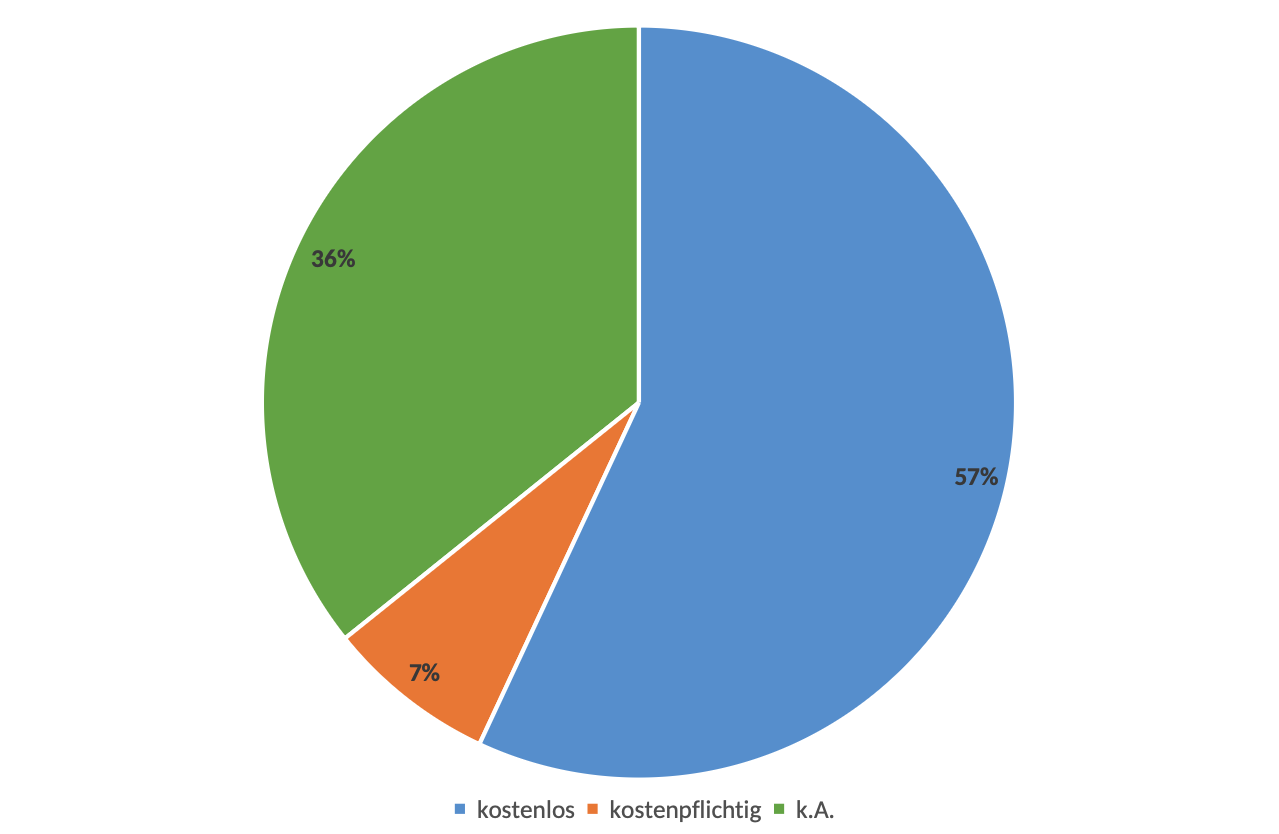
\includegraphics[width=0.9\textwidth]{graphics_lit/14-preis.png}
    \caption{Aufteilung Preis}
    \label{fig:14-preis2}
\end{figure}

\begin{figure}[!htbp]
    \centering
    % --- linke Seite: Grafik ---
    \begin{subfigure}[b]{0.48\textwidth}
        \centering
        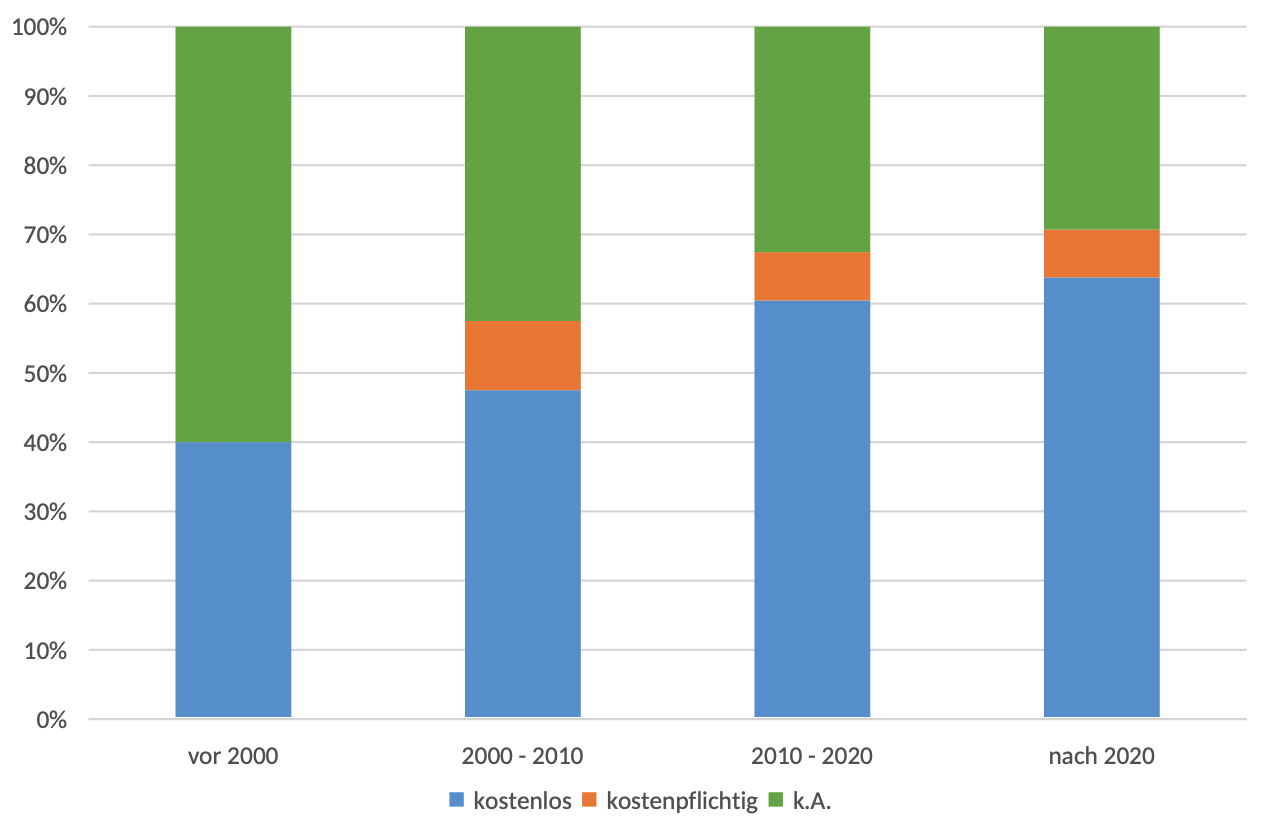
\includegraphics[width=\textwidth]{graphics_lit/15-preis-jahr.png}
        \caption{Aufteilung Preis (grafisch)}
        \label{fig:15-preis-jahr}
    \end{subfigure}
    \hfill
    % --- rechte Seite: Tabelle ---
    \begin{subfigure}[b]{0.48\textwidth}
        \centering
        \tiny
        \begin{tabularx}{\textwidth}{lXXX}
            \hline
            \textbf{Zeitraum} & \textbf{kostenlos} & \textbf{kostenpflichtig} & \textbf{k.A.} \\
            \hline
            vor 2000      & 4  & 0 & 6  \\
            2000--2010    & 19 & 4 & 17 \\
            2010--2020    & 26 & 3 & 14 \\
            nach 2020     & 37 & 4 & 17 \\
            \hline
        \end{tabularx}
        \caption{Aufteilung Preis (detailliert)}
        \label{tab:15-preis-zeit}
    \end{subfigure}
    %
    \caption{Darstellung der Preisgestaltung der Simulatoren über verschiedene Zeiträume}
    \label{fig:15-preis-gesamt}
\end{figure}

In Bezug auf das Kriterium \textit{Dokumentation} gibt Abbildung~\ref{fig:16-dokumentation} genauere Einblicke. In 87~\% der analysierten Publikationen verfügen die verwendeten bzw. beschriebenen Simulatoren über eine Dokumentation, während 5~\% keine Dokumentation erwähnen und in 7~\% der Publikationen hierzu keine Angaben vorliegen.

\begin{figure}[!htbp]
    \centering
    \caption{Aufteilung Dokumentation}
    \label{fig:16-dokumentation}
    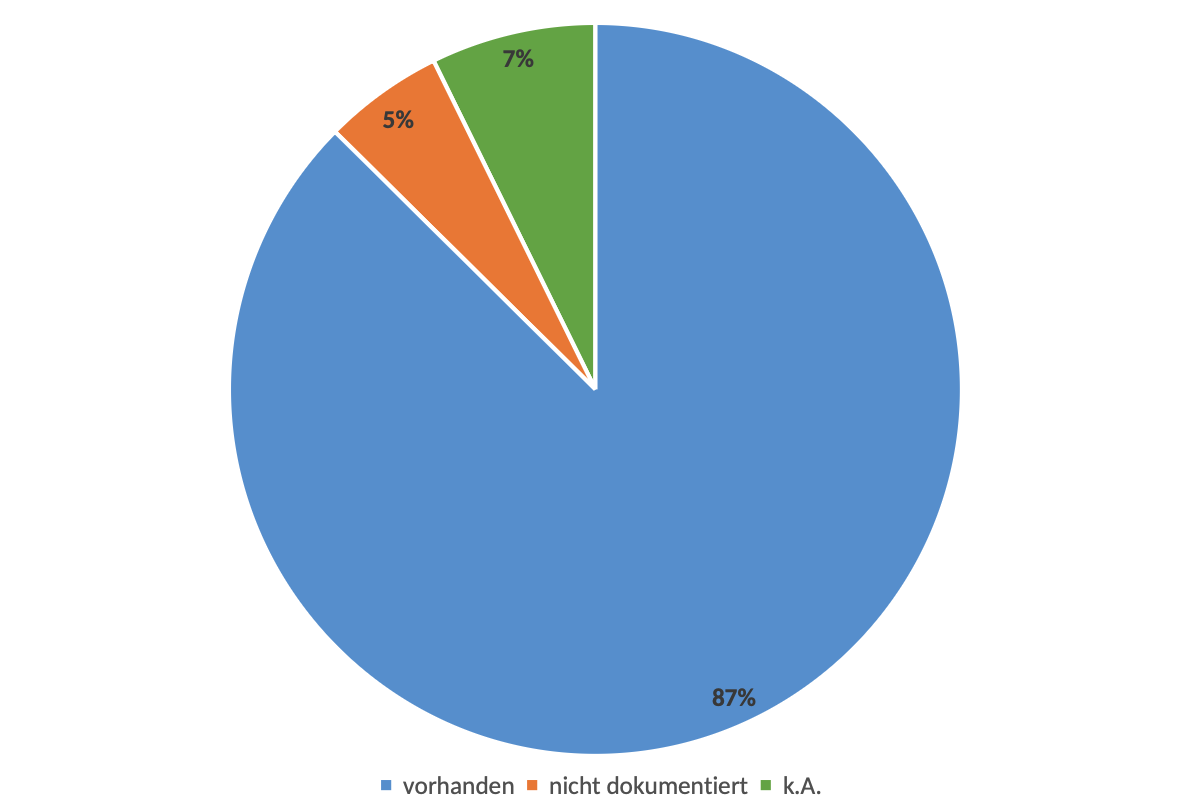
\includegraphics[width=0.90\textwidth]{graphics_lit/16-dokumentation.png}
\end{figure}

Als abschließendes Kriterium wird die Anzahl der Zitationen untersucht. Tabelle~\ref{tab:zitationen} zeigt die am häufigsten zitierten Publikationen pro Thema, da diese für weiterführende oder aufbauende Untersuchungen in den jeweiligen Bereichen als maßgeblich gelten. Die Auswahl der dargestellten Publikationen erfolgte auf Grundlage des Durchschnitts aller Zitationen, der bei etwa 35 liegt. Publikationen mit mehr als 35 Zitationen werden nachfolgend dargestellt.

{
\tiny
\centering
\begin{longtable}{|c|p{6cm}|p{3cm}|c|}
    \caption{Häufig zitierte Publikationen pro Themengebiet\label{tab:zitationen}} \\
    \hline
    \textbf{Zitationen} & \textbf{Titel} & \textbf{Autor(en)} & \textbf{Jahr} \\
    \hline
    \endfirsthead

    \hline
    \textbf{Zitationen} & \textbf{Titel} & \textbf{Autor(en)} & \textbf{Jahr} \\
    \hline
    \endhead

    \hline
    \multicolumn{4}{l}{Fortsetzung auf der nächsten Seite} \\
    \hline
    \endfoot

    \hline
    \endlastfoot

    % --- Inhalte ---
    \multicolumn{4}{c}{\textbf{AI}} \\
    \hline
    211 & Teaching CS50 with AI: Leveraging Generative Artificial Intelligence in Computer Science Education & R. Liu, C. Zenke, C. Liu, A. Holmes, P. Thornton, D. J. Malan & 2024 \\
    \hline
    \multicolumn{4}{c}{\textbf{GPU}} \\
    \hline
    146 & MGPUSim: Enabling Multi-GPU Performance Modeling and Optimization & Y. Sun, T. Baruah, S. A. Mojumber, S. Dong, X. Gong, S. Treadway & 2019 \\
    397 & Accel-Sim: An Extensible Simulation Framework for Validated GPU Modeling & M. Khairy, Z. Shen, T. M. Aamodt, T. G. Rogers & 2020 \\
    \hline
    \multicolumn{4}{c}{\textbf{Grundlagen und Theorien}} \\
    \hline
    117 & Flexible Web-Based Educational System for Teaching Computer Architecture and Organization & J. Djordjevic, B. Nikolic, A. Milenkovic & 2005 \\
    \hline
    \multicolumn{4}{c}{\textbf{Hardware und Logik}} \\
    \hline
    46 & Harnessing FPGAs for Computer Architecture Education & M. Holland, J. Harris, S. Hauck & 2003 \\
    \hline
    \multicolumn{4}{c}{\textbf{Programmierung}} \\
    \hline
    41 & Using Simulators for Teaching Computer Organization and Architecture & P. W. C. Prasad, A. Alsadoon, A. Beg, A. Chan & 2016 \\
    51 & MarieSim: The MARIE Computer Simulator & L. Null, J. Lobur & 2003 \\
    \hline
    \multicolumn{4}{c}{\textbf{Prozessoren und Architekturen}} \\
    \hline
    162 & Control Flow Modeling in Statistical Simulation for Accurate and Efficient Processor Design Studies & L. Eeckhout, R. H. Bell, B. Stougie, K. De Bosschere, L. K. John & 2004 \\
    172 & Applying a Constructivist and Collaborative Methodological Approach in Engineering Education & L. Moreno, C. Gonzalez, I. Castilla, E. Gonzalez, J. Sigue & 2007 \\
    327 & Measuring Experimental Error in Microprocessor Simulation & R. Desikan, D. Burger, S. W. Keckler & 2001 \\
    \hline
    \multicolumn{4}{c}{\textbf{Speicher und Performance}} \\
    \hline
    53 & Cryogenic Computer Architecture Modeling with Memory-Side Case Studies & L. Gyu-Hyeon, M. Dongmoon, B. Ilkwon, K. Jangwoo & 2019 \\
    205 & A Simulation Based Study of TLB Performance & A. Borg, J. B. Chen, N. P. Jouppi & 1992 \\
    \hline
    \multicolumn{4}{c}{\textbf{Systeme und Anwendungen}} \\
    \hline
    139 & Virtual Reality in Computer Science Education: A Systematic Review & J. Priker, A. Dengel, M. Holly, S. Safikani & 2020 \\
    \hline
\end{longtable}
}



